\documentclass[journal, a4paper]{IEEEtran}

\usepackage{graphicx}
\usepackage{url}
\usepackage{amsmath} 
\usepackage{booktabs}


%% Code Listing setup
\usepackage{listings}
\usepackage{color}

\definecolor{mygreen}{rgb}{0,0.6,0}
\definecolor{mygray}{rgb}{0.5,0.5,0.5}
\definecolor{mymauve}{rgb}{0.58,0,0.82}

\lstset{ %
  backgroundcolor=\color{white},   % choose the background color
  basicstyle=\footnotesize,        % size of fonts used for the code
  breaklines=true,                 % automatic line breaking only at whitespace
  captionpos=t,                    % sets the caption-position to bottom
  commentstyle=\color{mygreen},    % comment style
  escapeinside={\%*}{*)},          % if you want to add LaTeX within your code
  keywordstyle=\color{blue},       % keyword style
  stringstyle=\color{mymauve},     % string literal style
}

\def\arraystretch{1.25}


\begin{document}

	\title{Report on Implementation of Fast Multiplication Routines in Fortran}
	\author{B.Sc. Adam Kosiorek, M.Sc. Nils Zander}	
	\markboth{Institute for Computation in Engineering, Technische Universit\"at M\"unchen}{}
	\maketitle
	


\begin{abstract}
 This report describes the derivation of performance models and development of fast matrix multiplication routines in Fortran for Intel Xeon E5-2690 Sandy Bridge CPU for the ADHOC++ project.
\end{abstract}

\section{Introduction}
    \PARstart{T}{he} majority of numerically intensive software projects can be reduced on the lowest level to linear algebra problems. It is hardly surprising that the main suite of tools for them - Basic Linear Algebra Subroutines (BLAS) - is amongst the most heavily optimized software packages out there. Using advanced data distribution and load balancing techniques, it leverages data locality and various levels of parallelism to boost performance. Many BLAS implementations are, however, ill-suited for small sized problems. As shown later, Intel MKL~-- arguably the fastest implementation for x86 CPUs~\cite{MKL}~-- is easily outperformed by the most na\"ive general matrix-matrix multiplication code when inputs are not big enough. In many cases it is therefore possible and necessary to devise custom matrix multiplication routines optimized for smaller problems. We develop performance model and optimized code for the following cases of matrix-matrix multiplication:
    \begin{equation}
     C = Ax + C
    \end{equation}
    where $C \in \mathcal{R}^{N \times K}$, $A \in \mathcal{R}^{N \times M}$, $x \in \mathcal{R}^{M \times K}$ and $N \in \mathcal{N}^+$, $K \in \{1, 2, 3\}$


\section{Performance Model}
    Theoretical performance models, while not perfectly accurate, can hugely benefit development of optimized numerical programming routines by providing a maximum performance estimate as a goal to strive for. Maximum theoretical performance can be computed by: 
    \begin{equation}
     P_{peak} = IPC \cdot FPI \cdot Frequency
    \end{equation}
    where $IPC$ - instructions per cycle, $FPI$ - floating point operations per instruction, $Frequency$ - CPU's frequency. Intel Xeon E5-2690 operates with the frequency of $2.9$ GHz and is capable of executing 1, 2 or 4 $FPI$, depending on the operation mode (Scalar, SSE, AVX). $IPC$ depends on the numerical algorithm or the average number of floating point instructions executed per cycle to compute a single element of the output matrix. To derive $IPC$ and $P_{peak}$, we refer to table \ref{tab:low_level}, which lists instructions that can be executed in one cycle by the Sandy Bridge CPU and to table \ref{tab:req}, which depicts number of each low level instructions needed to be executed to compute one entry of $C$ matrix. Finally, table \ref{tab:perf} summarizes results. It is obvious that our case can hugely benefit from AVX operation mode.
    
      \begin{table}[!hbt]
	\begin{center}
	  \caption{Low level instructions per cycle.}
	  \label{tab:low_level}
	  \begin{tabular}{c|c|c}
		  Instruction	& Scalar & AVX \\
		  \hline
		  load		& 1 or 2 & 1 \\
		  \hline
		  store		& 1 or 0 & 0.5 \\
		  \hline
		  multiply	& 1 & 1 \\
		  \hline
		  add 		& 1 & 1 \\
	  \end{tabular}
	\end{center}
      \end{table}
      
      \begin{equation}      
	  K=1:\;\;C(i, 1) = C(i, 1) + A(i, 1) \cdot x(1, 1) 
      \end{equation} 
      
      \begin{equation}      
	\begin{split}
	  K=2:\;\;C(i, 1) = C(i, 1)  + A(i, 1) \cdot x(1, 1) \\+ A(i, 2) \cdot x(2, 1)
	\end{split}
      \end{equation}
      
      \begin{equation}      
	\begin{split}
	  K=3:\;\;C(i, 1) = C(i, 1) + A(i, 1) \cdot x(1, 1) \\+ A(i, 2) \cdot x(2, 1) \\+ A(i, 3) \cdot x(3, 1)
	\end{split}
      \end{equation}
      
  \begin{table}[!hbt]
    \begin{center}
      \caption{Low level instructions required to compute one entry of $C$ matrix.}
      \label{tab:req}
      \begin{tabular}{c|c|c|c|c}
	K	& load & store & multiply & add \\
	\hline
	1	& 2 & 1 & 1 & 1 \\
	\hline
	2	& 3 & 1 & 2 & 2 \\
	\hline
	3	& 4 & 1 & 3 & 3
      \end{tabular}
    \end{center}
  \end{table}
 
  \begin{table}[!hbt]
    \begin{center}
      \caption{Floating point instructions per cycle and peak theoretical performance for Scalar and AVX modes.}
      \label{tab:perf}
      \begin{tabular}{c|c|c|c|c}
		& \multicolumn{2}{c}{IPC} & \multicolumn{2}{c}{$P_{peak}$ [GFlops]} \\
	K	& Scalar & AVX	& Scalar & AVX \\
	\hline
	1	& 1 & 1 & 2.9 & 11.60 \\
	\hline
	2	& 2 & 1.33 & 5.8 & 15.47 \\
	\hline
	3	& 2 & 1.5 & 5.8 & 17.40
      \end{tabular}
    \end{center}
  \end{table}


\section{Implementation and Results}

  Fortran is the programming language traditionally used to implement high performance numerical algorithms. One reason is that it makes stronger assumptions about memory layout of variables than \textit{e.g.} the C language, thus making vectorization easier.  We decided to use Intel's Fortran compiler ifort, which often produces faster code than GNU's gfortran \cite{intel_comp}, but also provides easier to read and more complete optimization feedback. To use AVX instructions, we can rely on one of the following: (1) use compiler intrinsics or (2) write standard Fortran code in a way that enables automatic vectorization. The following sections describe constraints and counter-measures that enabled successful vectorization.
  
  \subsection{Memory Layout and Iteration}
    Fortran assumes column-major memory layout, that is, a single column of a matrix is comprised of elements adjacent in memory. In our case, the routines are executed from C/C++, which assumes row-major memory layout. Normally, that would require declaration of transposed matrices in Fortran: \textit{e.g.} \texttt{double A[sizeA1][sizeA2]} in C/C++ would become \texttt{DOUBLE PRECISION A(sizeA2, sizeA1)} in Fortran. Efficient multiplication, however, requires iteration along rows of the original matrices, which transfers to impossible to vectorize (\textit{i.e.} Scalar mode) iteration along the innermost dimension in Fortran. Thus, we resort to computing indices manually and declaring matrices as one dimensional vectors \textit{i.e.} \texttt{DOUBLE~PRECISION~A(sizeA1~$\cdot$~sizeA2)}. 
    
    This approach improves performance, but is still slow when compared to $P_{peak}$. A closer inspection of Assembly code reveals that AVX instructions are used, but inefficiently for $M > 1$. To understand it, we have to explicitly look at the data layout in memory. Equation \ref{eq:mat} represents the case of $M = 3$ as seen in Fortran (vector $C$ omitted for brevity).
    
  \begin{equation}
    x^TA^T = \begin{pmatrix}
	  x_1 & x_2 & x_3
	  \end{pmatrix}
	  \begin{pmatrix}
	    a_{1, 1} & a_{1, 2} & a_{1, 3} & \cdots \\
	    a_{2, 1} & a_{2, 2} & a_{2, 3} & \cdots \\
	    a_{3, 1} & a_{3, 2} & a_{3, 3} & \cdots \\
	  \end{pmatrix}
	  \label{eq:mat}
  \end{equation}

  Here, elements $a_{1, i}$, $a_{2, i}$, $a_{3, i}$ are contiguous in memory. Since AVX operates on 4 elements at once and only 3 elements are available, one element would have to be discarded. Compiler, therefore, chooses another way by unrolling the multiplication loop four times and vectorizing along the rows of the matrix. Now, four elements of C can be computed in three steps (using $a_{1, i:i+4}$ first, $a_{2, i:i+4}$ next and finally $a_{3, i:i+4}$). An inevitable performance loss occurs due to the elements $a_{j, i:i+4}$ being non-contiguous, so they have to be loaded one by one into the AVX register.    
    
\begin{equation}
  Ax = 
        \begin{pmatrix}
          a_{1, 1} & a_{1, 2} & a_{1, 3} \\
          a_{2, 1} & a_{2, 2} & a_{2, 3} \\
          a_{3, 1} & a_{3, 2} & a_{3, 3} \\
          \vdots & \vdots & \vdots \\
        \end{pmatrix}
        \begin{pmatrix}
         x_1 \\ x_2 \\ x_3
        \end{pmatrix}
        \label{eq:mat_transposed}
\end{equation}

  The opposite situation occurs with the transposed version of the problem, as shown in equation \ref{eq:mat_transposed}. Again, computation of one element of the $C$ vector would be inefficient, because one entry would have to be discarded from the AVX register. When unrolled 4 times, however, vectorization can proceed along memory-contiguous columns. Packed AVX load instructions lead to higher performance. 
    
  \subsection{Data Alignment}
    Another limiting factor is memory alignment. High performance AVX instructions can be used only when data are aligned at appropriate memory boundaries. Even if that is the case, the compiler cannot be sure if every possible input will be memory-aligned. One way to ensure it is to use inline compiler directives, in this case: \texttt{!DEC\$ VECTOR ALIGNED} just before vector references.
  
  \subsection{Data Dependency - Read after Write}
    Listing \ref{lst:raw} contains the Read after Write dependency. It prevents vectorization, since the same element in memory is referenced multiple times. One possible solution is to introduce a local variable that would accumulate the results and store it in \texttt{C(i)} only once as in listing \ref{lst:noraw}. The compiler than unrolls the outer loop with the code from listing \ref{lst:noraw} and vectorizes the result.
    \begin{lstlisting}[language=Fortran,label=lst:raw, caption=Read after Write dependency.]
      DO i = 1, 3
	C(i) = C(i) + A(index + i) * x(i)
      END DO
    \end{lstlisting}
    
    \begin{lstlisting}[language=Fortran,label=lst:noraw, caption=Read after Write dependency resolved.]
      sum = 0
      DO i = 1, 3
	sum = sum + A(index + i) * x(i)
      END DO
      C(i) = C(i) + sum
    \end{lstlisting}
    
    This optimization is relevant only to the normal (\textit{i.e}. non-transposed) setting.
    
   \subsection{Results}  
    Achieved results, summarized in table \ref{tab:results}, are not perfect and are true only for matrices small enough to fit in L2 cache. Divergence of theoretical and achieved results might stem from the fact that we did not consider memory bandwidth or cache effects. They also suggest that using transposed matrix $A$ might be extremely beneficial in terms of speed. Even performing transposition before multiplication could be justified when a number of different $x$ vectors is to be multiplied. Figures \ref{fig:1x1}, \ref{fig:2x1} and \ref{fig:3x1} compare performance of multiplication routines of the normal and transposed cases with Intel's MKL. MKL's functions \texttt{cblas\_daxpy} was used for \texttt{[1x1]} case and \texttt{cblas\_dgemv} for cases \texttt{[2x1]} and \texttt{[3x1]}.
  
  \begin{table}[!hbt]
    \begin{center}
      \caption{Achieved results and comparison with theoretical peak performance}
      \label{tab:results}
      \begin{tabular}{c|c|c}
	K	& $P_{achieved}$ [Gflops] & $P_{achieved} / P_{peak}$\\
	\hline
	$1$	& 9.17 & 0.79 \\
	\hline
	$2$	& 9.64 & 0.62 \\
	\hline
	$3$	& 7.15 & 0.41 \\
	\hline
	$2^T$	& 11.89 & 0.77 \\
	\hline
	$3^T$	& 13.96 & 0.8 \\
      \end{tabular}
    \end{center}
  \end{table}
  
  
  \begin{figure}
   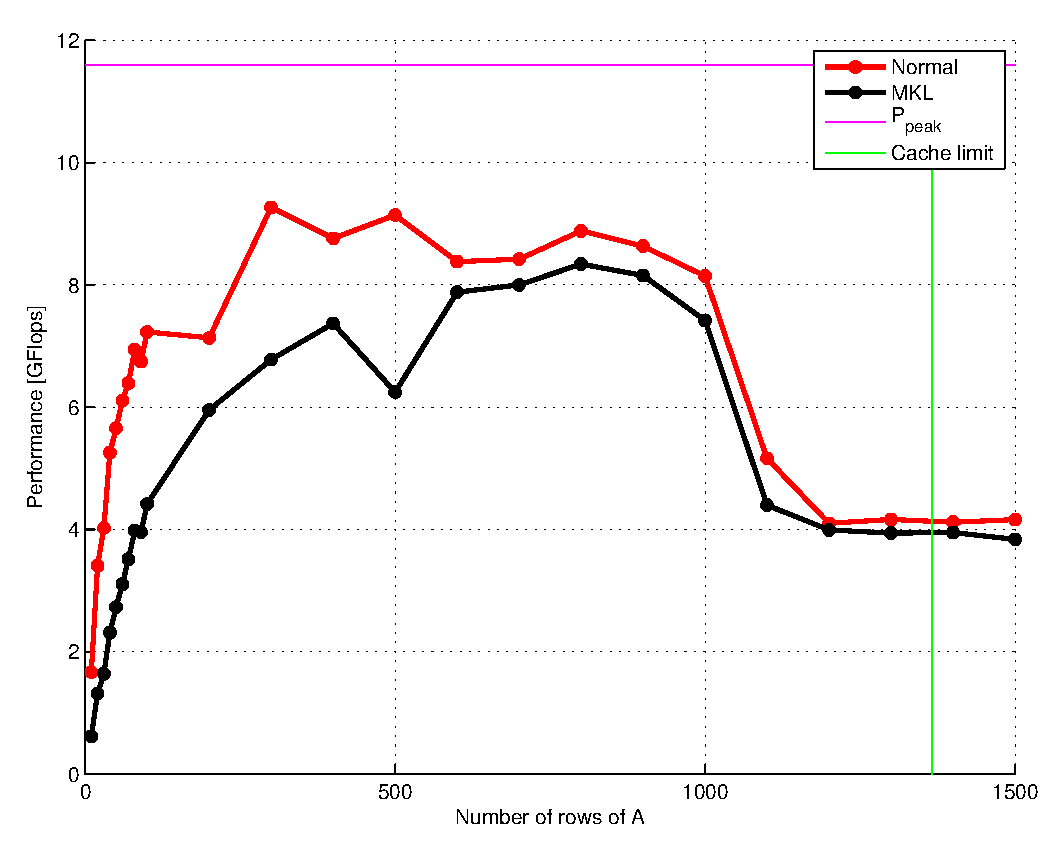
\includegraphics[width=0.5\textwidth]{1x1}
   \caption{Performance of $C = Ax + C$, where $x \in \mathcal{R}$}
   \label{fig:1x1}
  \end{figure}
  
  \begin{figure}
   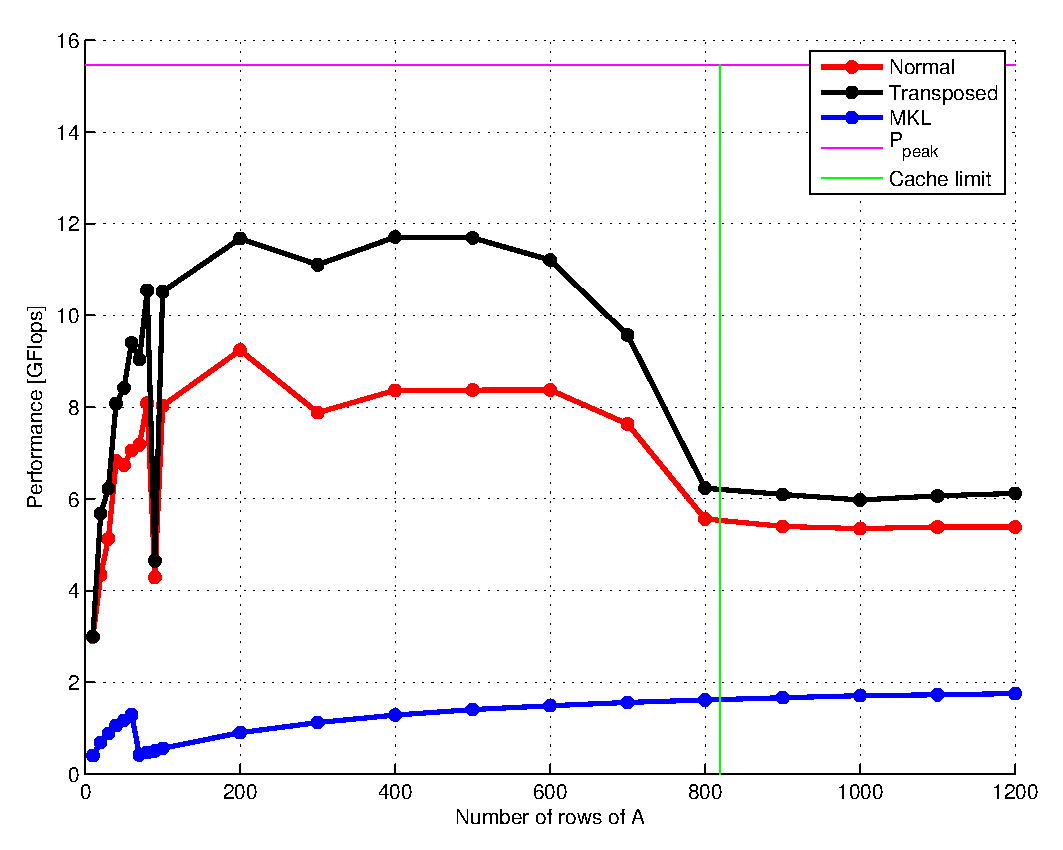
\includegraphics[width=0.5\textwidth]{2x1}
   \caption{Performance of $C = Ax + C$, where $x \in \mathcal{R}^{2\times 1}$}
   \label{fig:2x1}
  \end{figure}
  
  \begin{figure}
   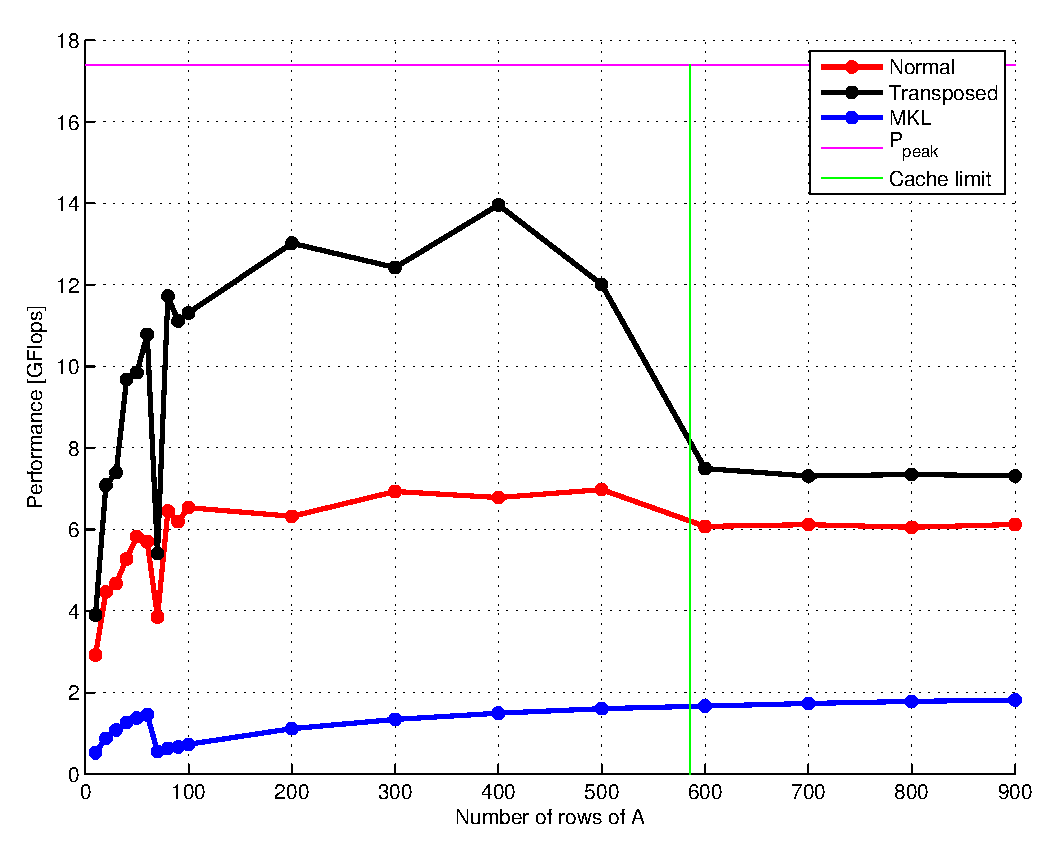
\includegraphics[width=0.5\textwidth]{3x1}
   \caption{Performance of $C = Ax + C$, where $x \in \mathcal{R}^{3\times 1}$}
   \label{fig:3x1}
  \end{figure}

   


\begin{thebibliography}{5}
	
	\bibitem{MKL}
	Intel Math Kernel Library: \url{https://software.intel.com/en-us/intel-mkl}
	
	\bibitem{intel_comp}
	Intel® Parallel Studio XE 2015 Product Brief: \url{https://goo.gl/vc5eYo}

\end{thebibliography}

% Your document ends here!
\end{document}
